\documentclass[11pt]{article}
\usepackage[textwidth=18.0cm, textheight=23.0cm, top=2.0cm]{geometry}
\usepackage{pst-all}
\usepackage{amssymb}
\usepackage{tikz}
\usepackage{underscore}\begin{document}
\pagestyle{empty}


ClassName: \underline{\textbf{Class_08.2bp-11}}
\par
BinSize: \underline{\textbf{100 × 100}}
\par
ReduceSize: \underline{\textbf{100 × 100}}
\par
TypeNum: \underline{\textbf{40}}
\par
Num: \underline{\textbf{40}}
\par
OutS: \underline{\textbf{130000}}
\par
InS: \underline{\textbf{106455}}
\par
Rate: \underline{\textbf{0.819}}
\par
UB: \underline{\textbf{13}}
\par
LB0: \underline{\textbf{13}}
\par
LB: \underline{\textbf{13}}
\par
LBWithCut: \underline{\textbf{13}}
\par
NodeCut: \underline{\textbf{0}}
\par
ExtendedNodeCnt: \underline{\textbf{1}}
\par
GenNodeCnt: \underline{\textbf{1}}
\par
PrimalNode: \underline{\textbf{0}}
\par
ColumnCount: \underline{\textbf{13}}
\par
TotalCutCount: \underline{\textbf{0}}
\par
RootCutCount: \underline{\textbf{0}}
\par
LPSolverCnt: \underline{\textbf{1}}
\par
PricingSolverCnt: \underline{\textbf{0}}
\par
BranchAndBoundNum: \underline{\textbf{1}}
\par
isOpt: \underline{\textbf{true}}
\par
TimeOnInitSolution: \underline{\textbf{600.000 s}}
\par
TimeOnPrimal: \underline{\textbf{0.000 s}}
\par
TimeOnPricing: \underline{\textbf{0.000 s}}
\par
TimeOnRmp: \underline{\textbf{0.078 s}}
\par
TotalTime: \underline{\textbf{600.344 s}}
\par
\newpage


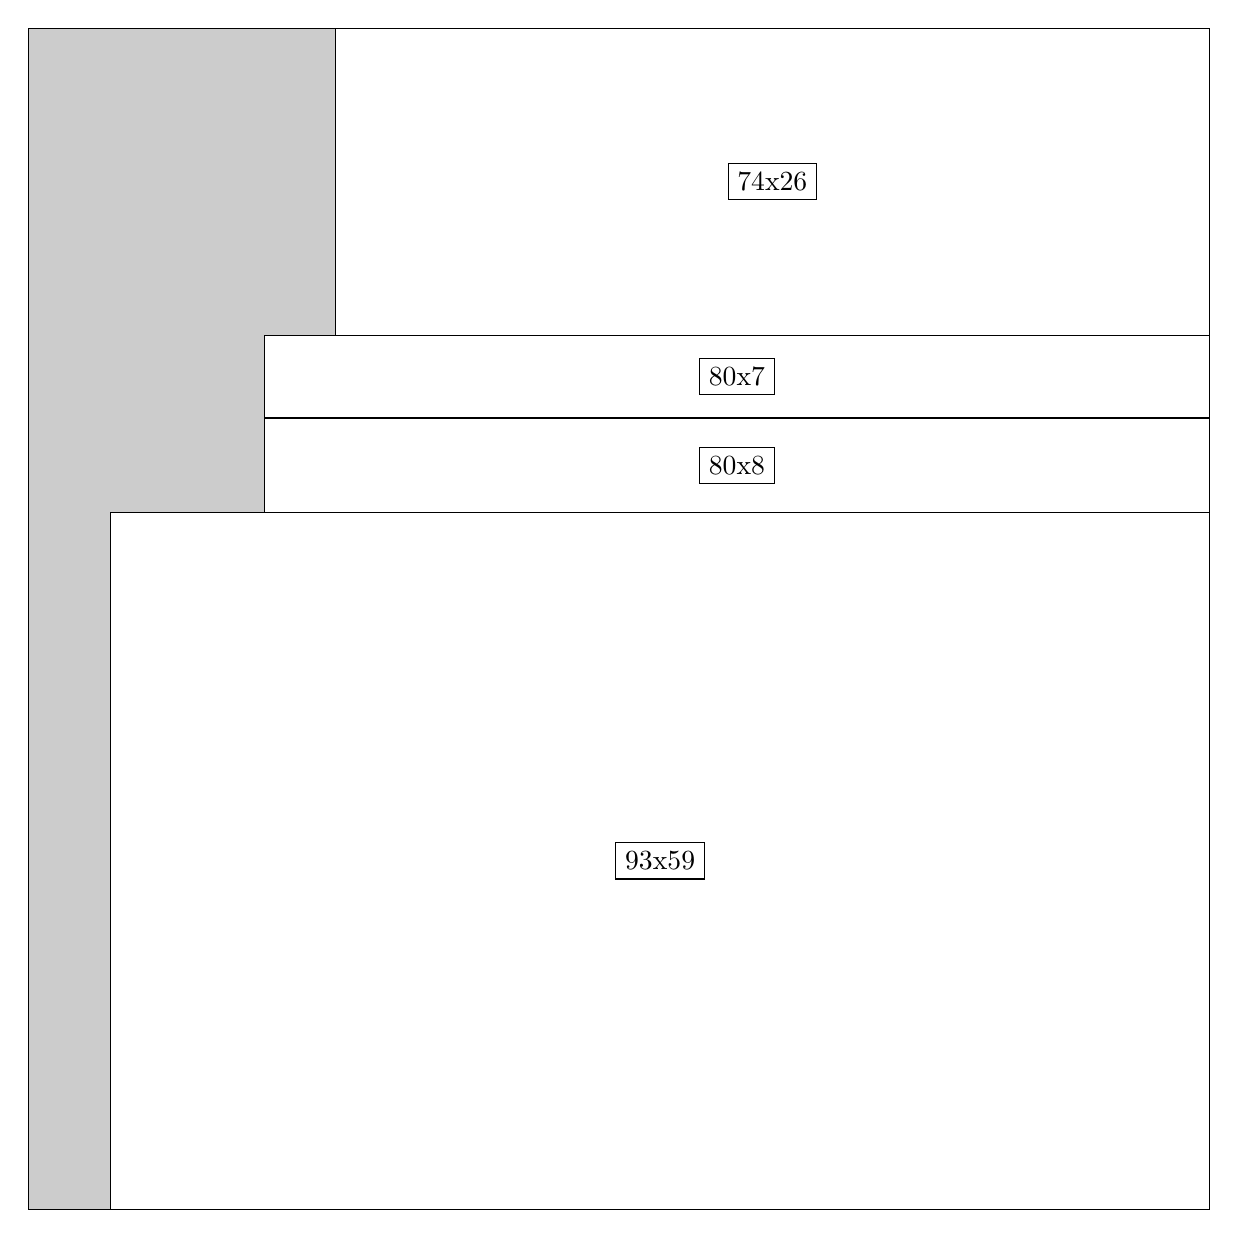
\begin{tikzpicture}[shorten >=1pt,scale=1.0,every node/.style={scale=1.0},->]
\tikzstyle{vertex}=[circle,fill=black!25,minimum size=14pt,inner sep=0pt]
\filldraw[fill=gray!40!white, draw=black] (0,0) rectangle (15.0,15.0);
\foreach \name/\x/\y/\w/\h in {93x59/1.05/0.0/13.95/8.85,80x8/3.0/8.85/12.0/1.2,80x7/3.0/10.049999999999999/12.0/1.05,74x26/3.9/11.1/11.1/3.9}
\filldraw[fill=white!40!white, draw=black] (\x,\y) rectangle node[draw] (\name) {\name} ++(\w,\h);
\end{tikzpicture}


w =93 , h =59 , x =7 , y =0 , v =5487
\par
w =80 , h =8 , x =20 , y =59 , v =640
\par
w =80 , h =7 , x =20 , y =67 , v =560
\par
w =74 , h =26 , x =26 , y =74 , v =1924
\par
\newpage


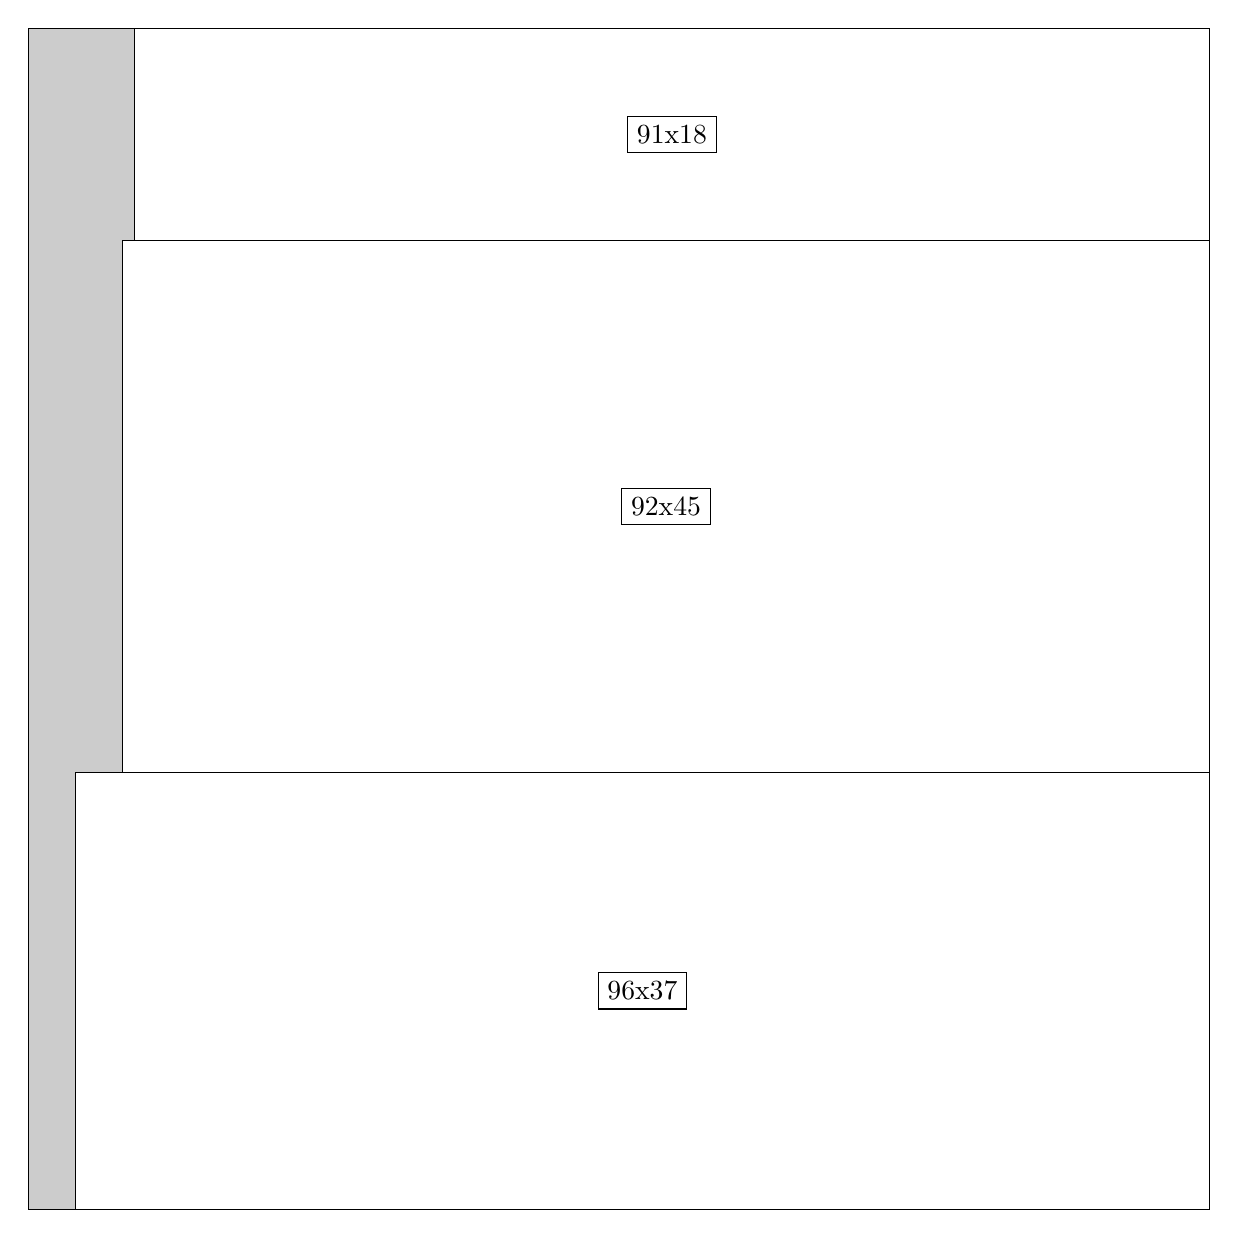
\begin{tikzpicture}[shorten >=1pt,scale=1.0,every node/.style={scale=1.0},->]
\tikzstyle{vertex}=[circle,fill=black!25,minimum size=14pt,inner sep=0pt]
\filldraw[fill=gray!40!white, draw=black] (0,0) rectangle (15.0,15.0);
\foreach \name/\x/\y/\w/\h in {96x37/0.6/0.0/14.399999999999999/5.55,92x45/1.2/5.55/13.799999999999999/6.75,91x18/1.3499999999999999/12.299999999999999/13.65/2.6999999999999997}
\filldraw[fill=white!40!white, draw=black] (\x,\y) rectangle node[draw] (\name) {\name} ++(\w,\h);
\end{tikzpicture}


w =96 , h =37 , x =4 , y =0 , v =3552
\par
w =92 , h =45 , x =8 , y =37 , v =4140
\par
w =91 , h =18 , x =9 , y =82 , v =1638
\par
\newpage



\begin{tikzpicture}[shorten >=1pt,scale=1.0,every node/.style={scale=1.0},->]
\tikzstyle{vertex}=[circle,fill=black!25,minimum size=14pt,inner sep=0pt]
\filldraw[fill=gray!40!white, draw=black] (0,0) rectangle (15.0,15.0);
\foreach \name/\x/\y/\w/\h in {89x95/1.65/0.0/13.35/14.25}
\filldraw[fill=white!40!white, draw=black] (\x,\y) rectangle node[draw] (\name) {\name} ++(\w,\h);
\end{tikzpicture}


w =89 , h =95 , x =11 , y =0 , v =8455
\par
\newpage


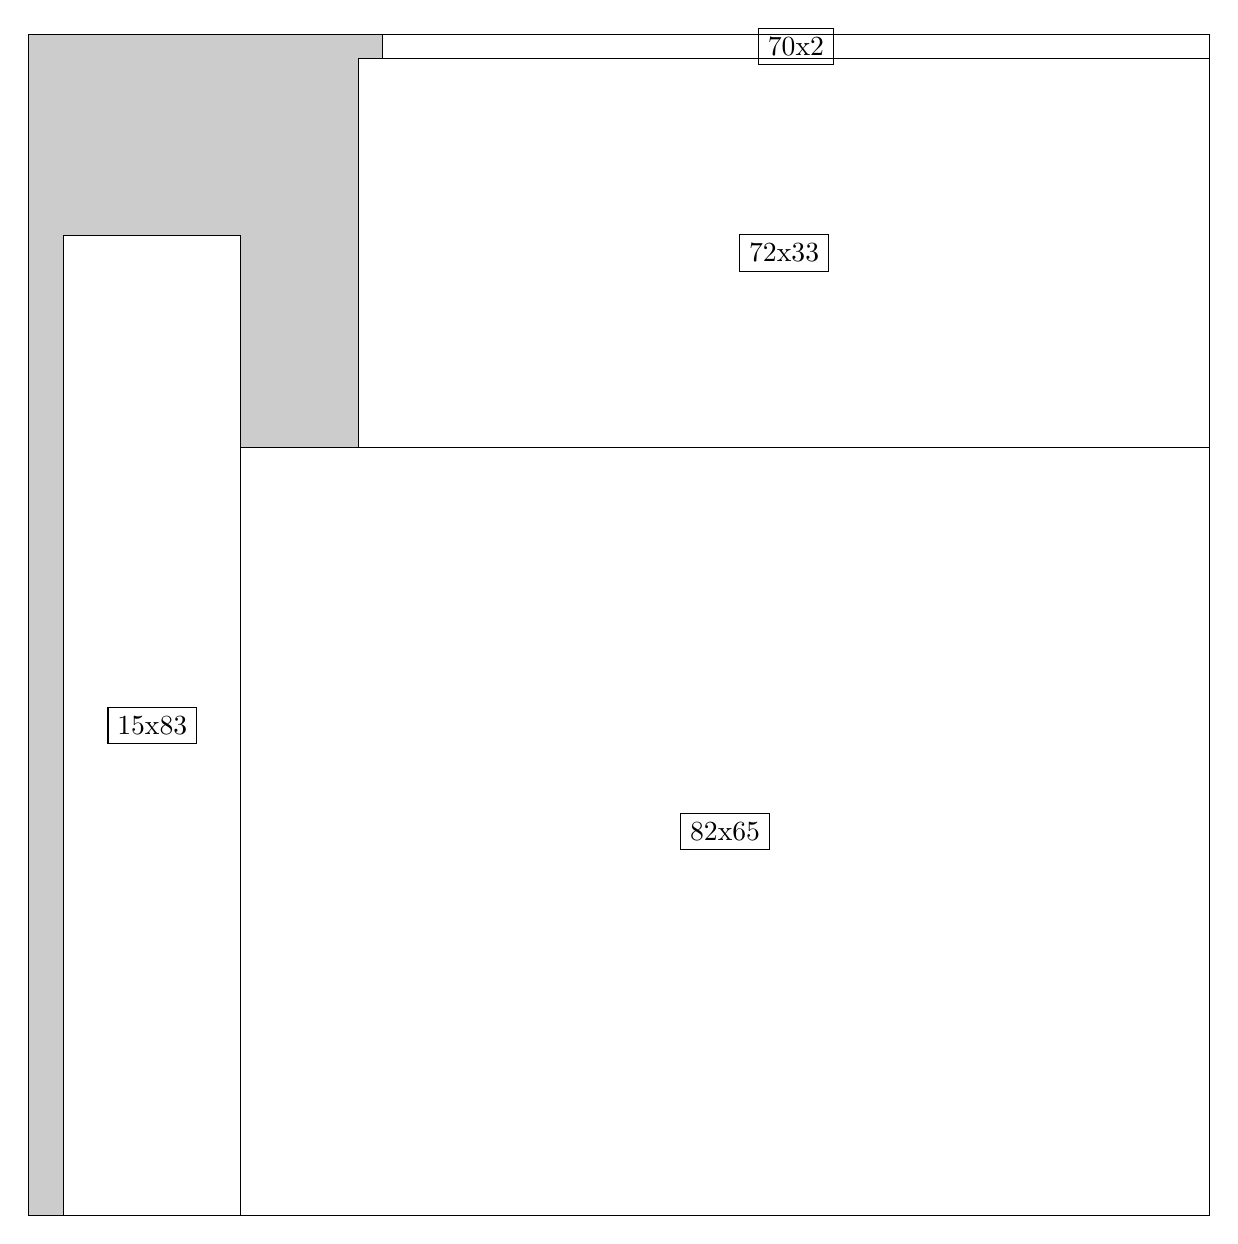
\begin{tikzpicture}[shorten >=1pt,scale=1.0,every node/.style={scale=1.0},->]
\tikzstyle{vertex}=[circle,fill=black!25,minimum size=14pt,inner sep=0pt]
\filldraw[fill=gray!40!white, draw=black] (0,0) rectangle (15.0,15.0);
\foreach \name/\x/\y/\w/\h in {82x65/2.6999999999999997/0.0/12.299999999999999/9.75,72x33/4.2/9.75/10.799999999999999/4.95,70x2/4.5/14.7/10.5/0.3,15x83/0.44999999999999996/0.0/2.25/12.45}
\filldraw[fill=white!40!white, draw=black] (\x,\y) rectangle node[draw] (\name) {\name} ++(\w,\h);
\end{tikzpicture}


w =82 , h =65 , x =18 , y =0 , v =5330
\par
w =72 , h =33 , x =28 , y =65 , v =2376
\par
w =70 , h =2 , x =30 , y =98 , v =140
\par
w =15 , h =83 , x =3 , y =0 , v =1245
\par
\newpage


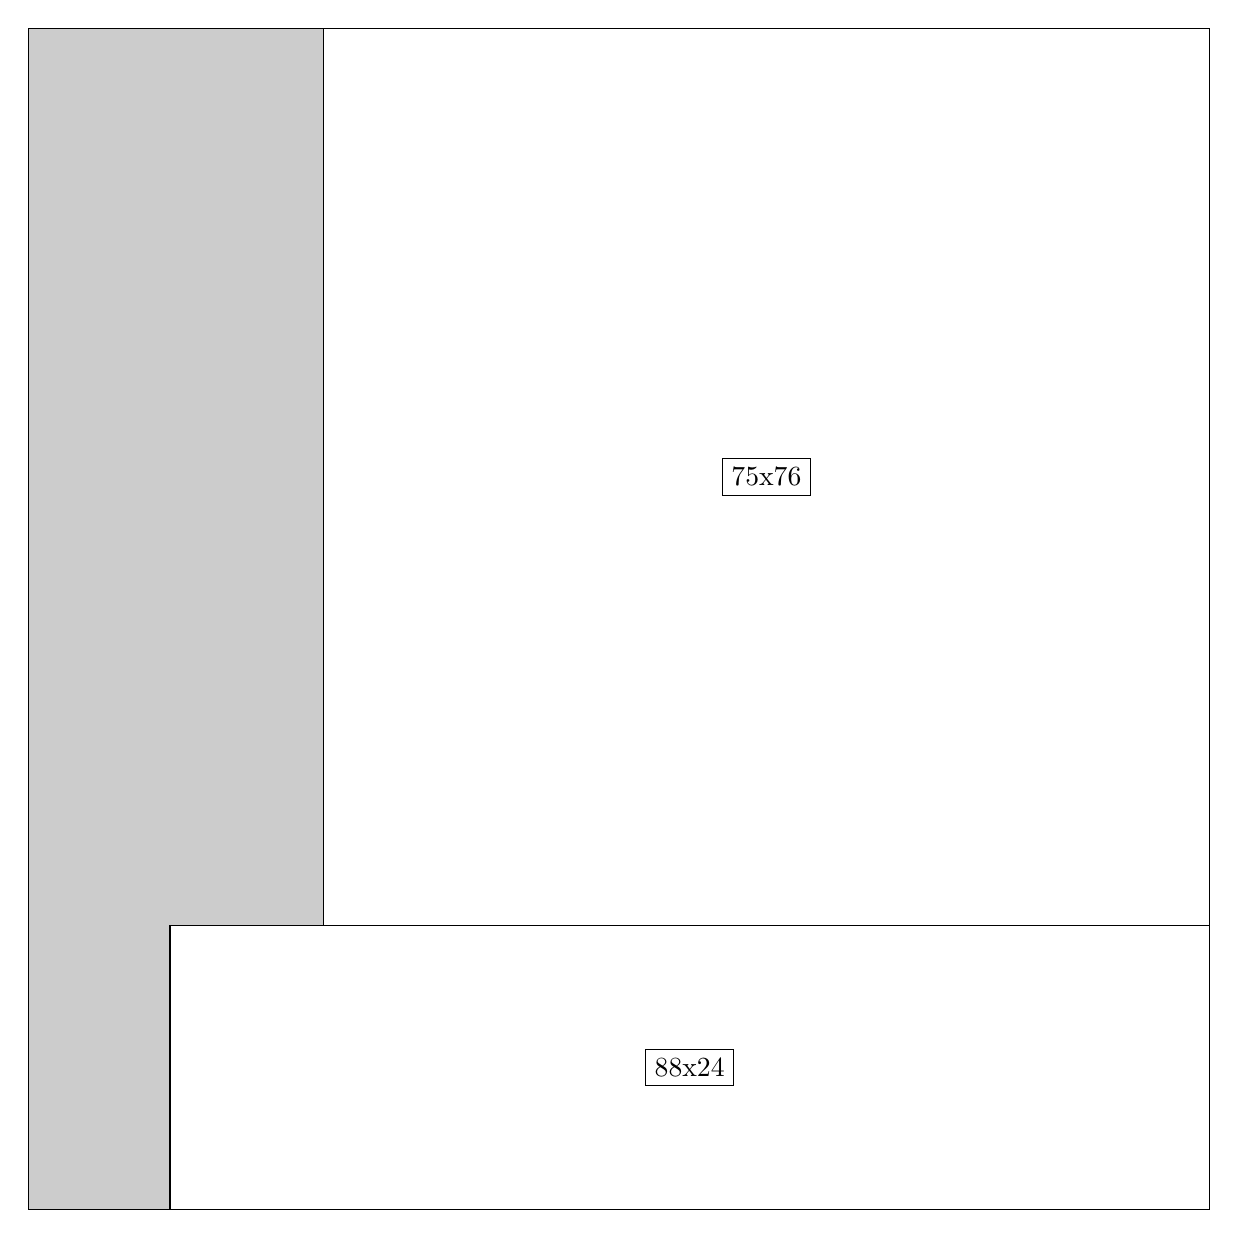
\begin{tikzpicture}[shorten >=1pt,scale=1.0,every node/.style={scale=1.0},->]
\tikzstyle{vertex}=[circle,fill=black!25,minimum size=14pt,inner sep=0pt]
\filldraw[fill=gray!40!white, draw=black] (0,0) rectangle (15.0,15.0);
\foreach \name/\x/\y/\w/\h in {88x24/1.7999999999999998/0.0/13.2/3.5999999999999996,75x76/3.75/3.5999999999999996/11.25/11.4}
\filldraw[fill=white!40!white, draw=black] (\x,\y) rectangle node[draw] (\name) {\name} ++(\w,\h);
\end{tikzpicture}


w =88 , h =24 , x =12 , y =0 , v =2112
\par
w =75 , h =76 , x =25 , y =24 , v =5700
\par
\newpage


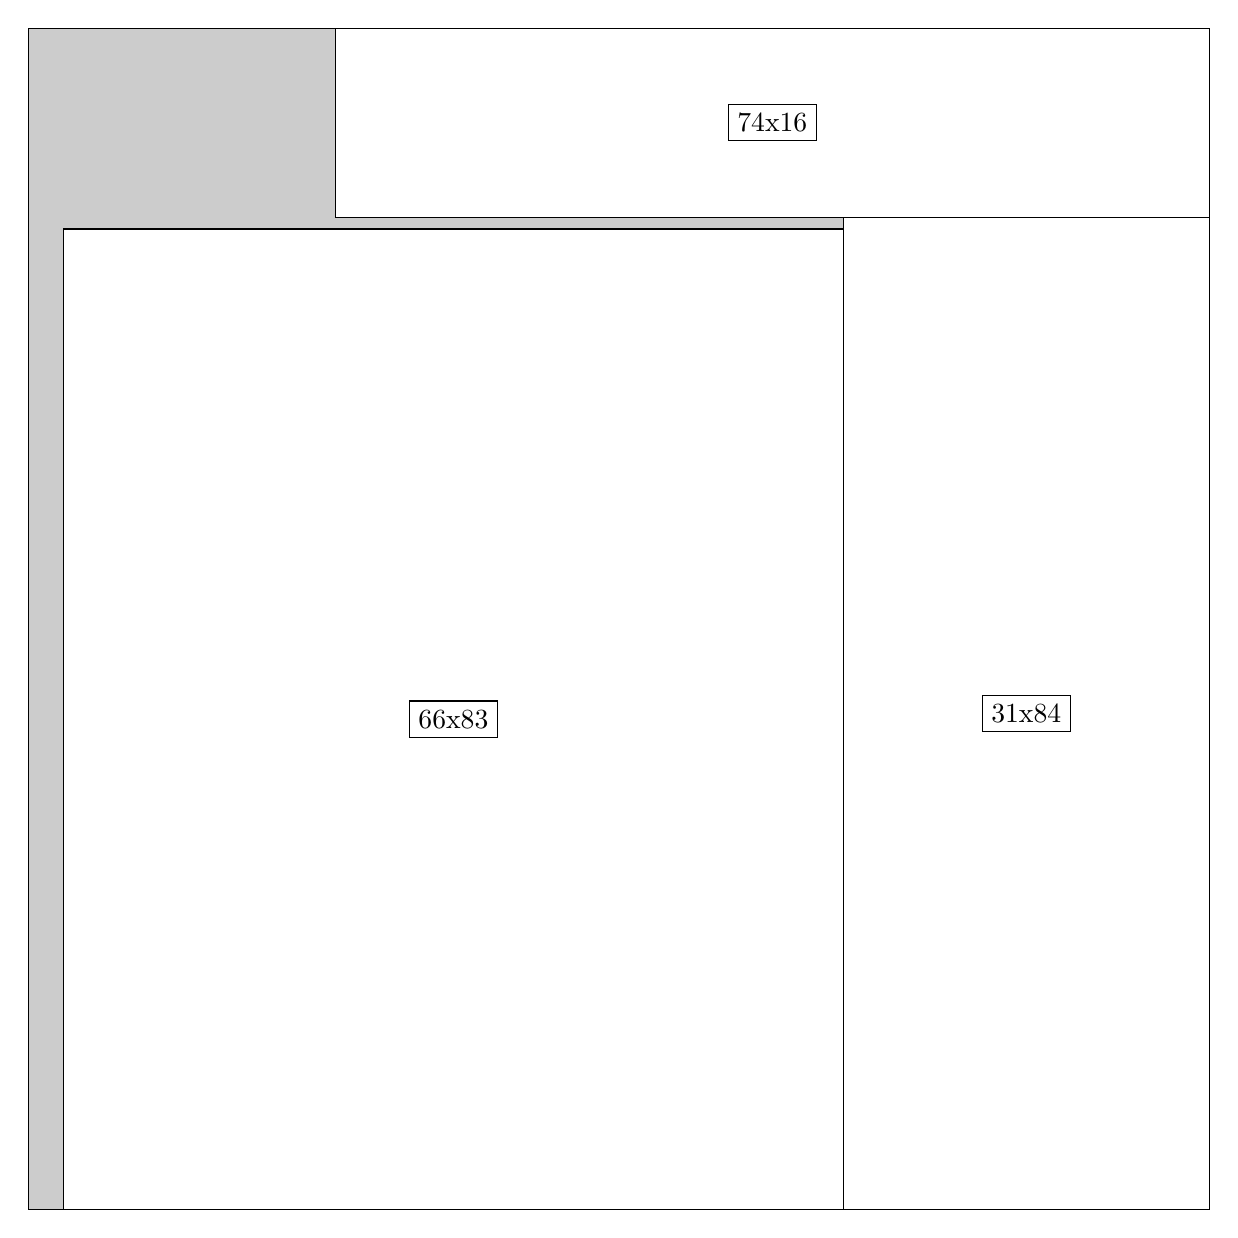
\begin{tikzpicture}[shorten >=1pt,scale=1.0,every node/.style={scale=1.0},->]
\tikzstyle{vertex}=[circle,fill=black!25,minimum size=14pt,inner sep=0pt]
\filldraw[fill=gray!40!white, draw=black] (0,0) rectangle (15.0,15.0);
\foreach \name/\x/\y/\w/\h in {31x84/10.35/0.0/4.6499999999999995/12.6,66x83/0.44999999999999996/0.0/9.9/12.45,74x16/3.9/12.6/11.1/2.4}
\filldraw[fill=white!40!white, draw=black] (\x,\y) rectangle node[draw] (\name) {\name} ++(\w,\h);
\end{tikzpicture}


w =31 , h =84 , x =69 , y =0 , v =2604
\par
w =66 , h =83 , x =3 , y =0 , v =5478
\par
w =74 , h =16 , x =26 , y =84 , v =1184
\par
\newpage


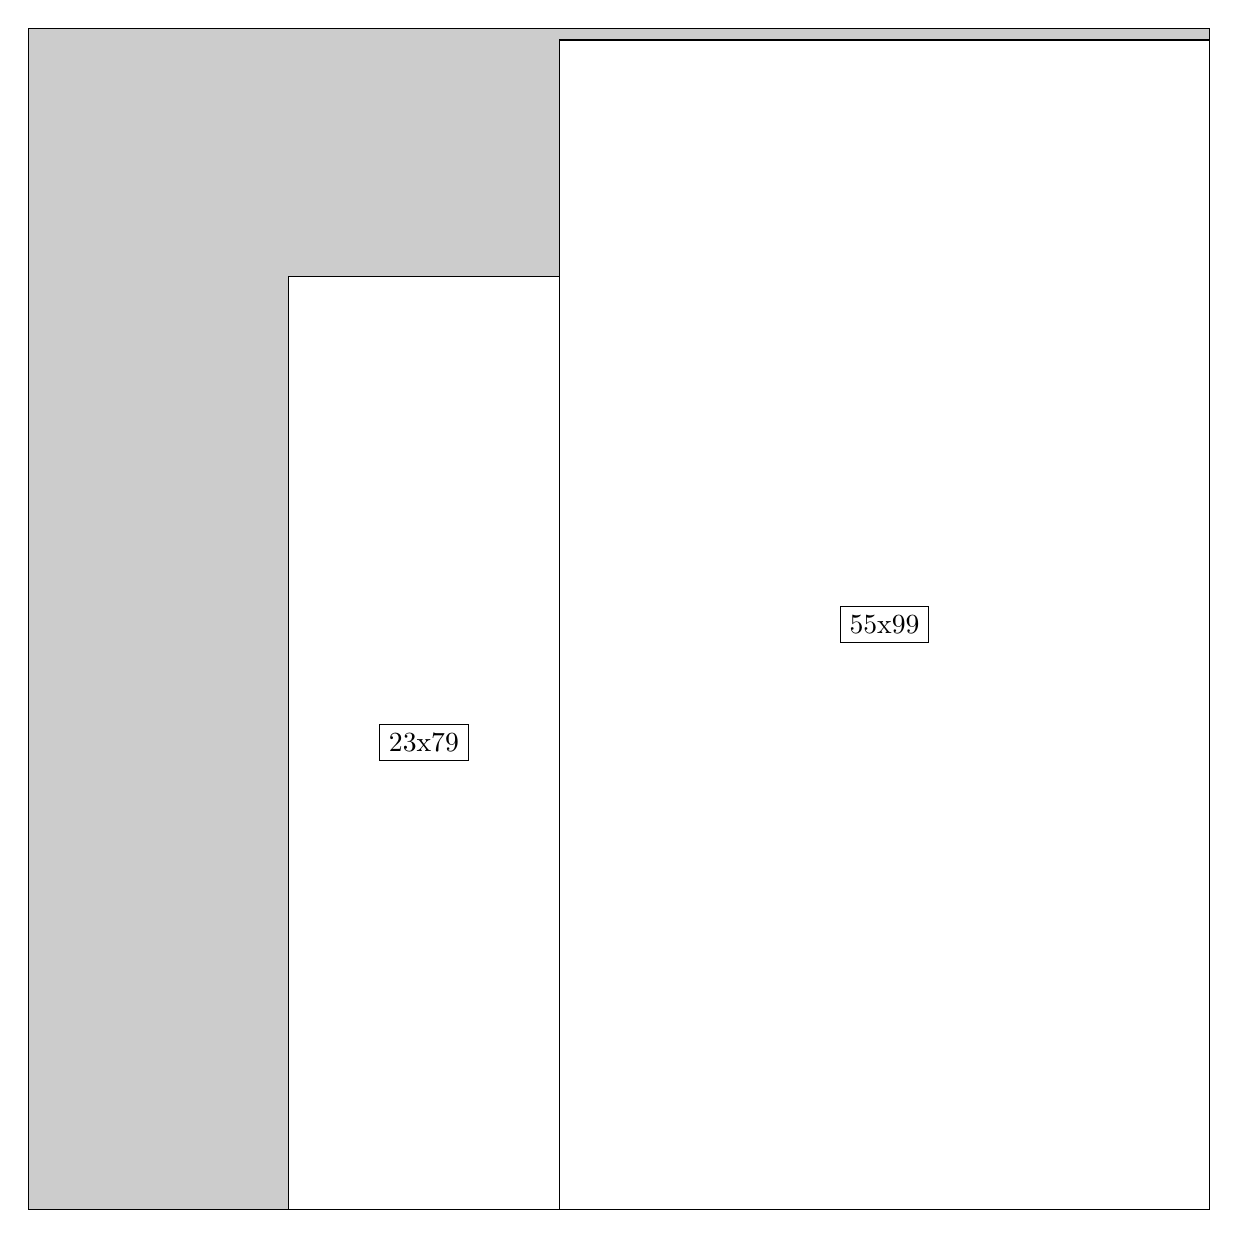
\begin{tikzpicture}[shorten >=1pt,scale=1.0,every node/.style={scale=1.0},->]
\tikzstyle{vertex}=[circle,fill=black!25,minimum size=14pt,inner sep=0pt]
\filldraw[fill=gray!40!white, draw=black] (0,0) rectangle (15.0,15.0);
\foreach \name/\x/\y/\w/\h in {55x99/6.75/0.0/8.25/14.85,23x79/3.3/0.0/3.4499999999999997/11.85}
\filldraw[fill=white!40!white, draw=black] (\x,\y) rectangle node[draw] (\name) {\name} ++(\w,\h);
\end{tikzpicture}


w =55 , h =99 , x =45 , y =0 , v =5445
\par
w =23 , h =79 , x =22 , y =0 , v =1817
\par
\newpage


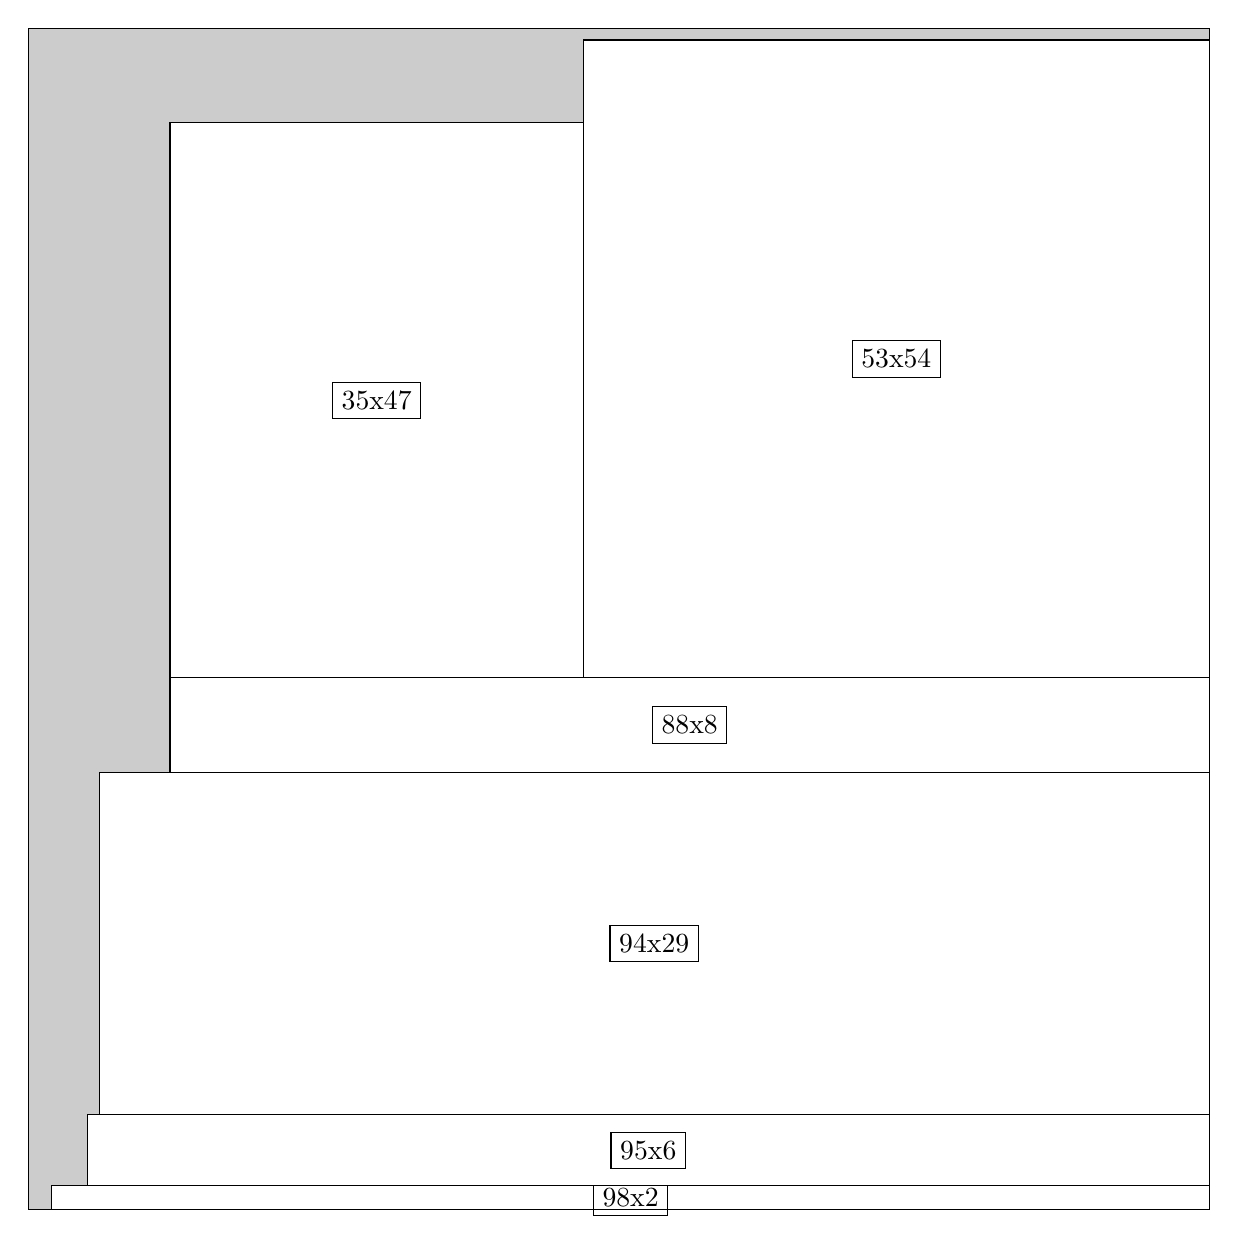
\begin{tikzpicture}[shorten >=1pt,scale=1.0,every node/.style={scale=1.0},->]
\tikzstyle{vertex}=[circle,fill=black!25,minimum size=14pt,inner sep=0pt]
\filldraw[fill=gray!40!white, draw=black] (0,0) rectangle (15.0,15.0);
\foreach \name/\x/\y/\w/\h in {98x2/0.3/0.0/14.7/0.3,95x6/0.75/0.3/14.25/0.8999999999999999,94x29/0.8999999999999999/1.2/14.1/4.35,88x8/1.7999999999999998/5.55/13.2/1.2,53x54/7.05/6.75/7.949999999999999/8.1,35x47/1.7999999999999998/6.75/5.25/7.05}
\filldraw[fill=white!40!white, draw=black] (\x,\y) rectangle node[draw] (\name) {\name} ++(\w,\h);
\end{tikzpicture}


w =98 , h =2 , x =2 , y =0 , v =196
\par
w =95 , h =6 , x =5 , y =2 , v =570
\par
w =94 , h =29 , x =6 , y =8 , v =2726
\par
w =88 , h =8 , x =12 , y =37 , v =704
\par
w =53 , h =54 , x =47 , y =45 , v =2862
\par
w =35 , h =47 , x =12 , y =45 , v =1645
\par
\newpage


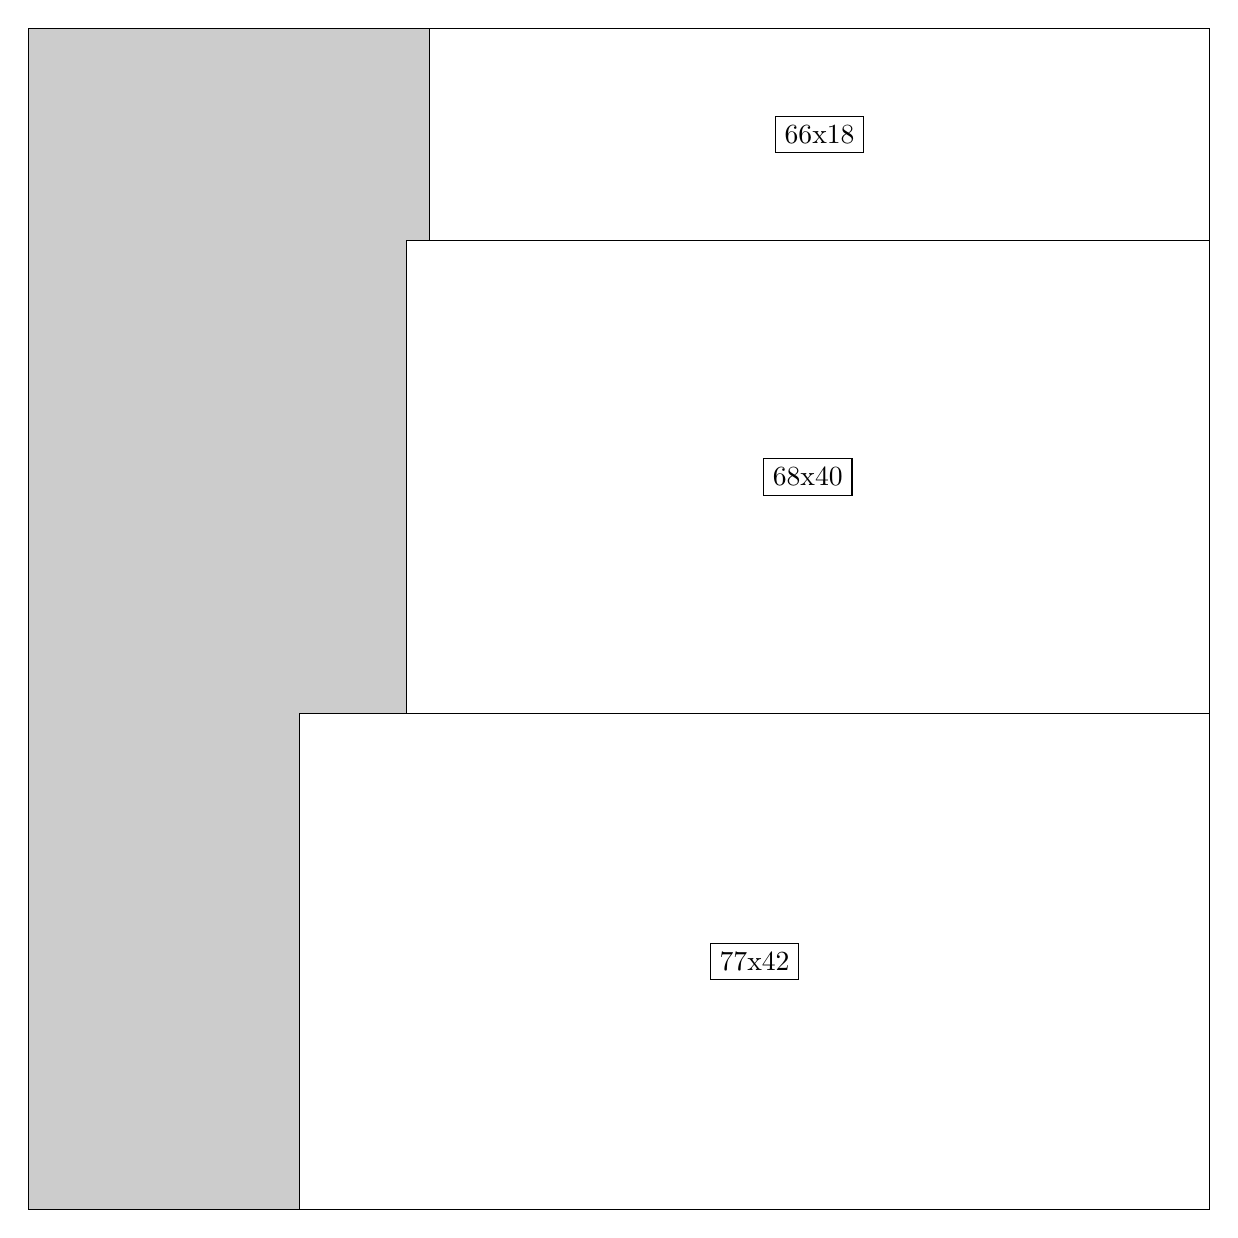
\begin{tikzpicture}[shorten >=1pt,scale=1.0,every node/.style={scale=1.0},->]
\tikzstyle{vertex}=[circle,fill=black!25,minimum size=14pt,inner sep=0pt]
\filldraw[fill=gray!40!white, draw=black] (0,0) rectangle (15.0,15.0);
\foreach \name/\x/\y/\w/\h in {77x42/3.4499999999999997/0.0/11.549999999999999/6.3,68x40/4.8/6.3/10.2/6.0,66x18/5.1/12.299999999999999/9.9/2.6999999999999997}
\filldraw[fill=white!40!white, draw=black] (\x,\y) rectangle node[draw] (\name) {\name} ++(\w,\h);
\end{tikzpicture}


w =77 , h =42 , x =23 , y =0 , v =3234
\par
w =68 , h =40 , x =32 , y =42 , v =2720
\par
w =66 , h =18 , x =34 , y =82 , v =1188
\par
\newpage


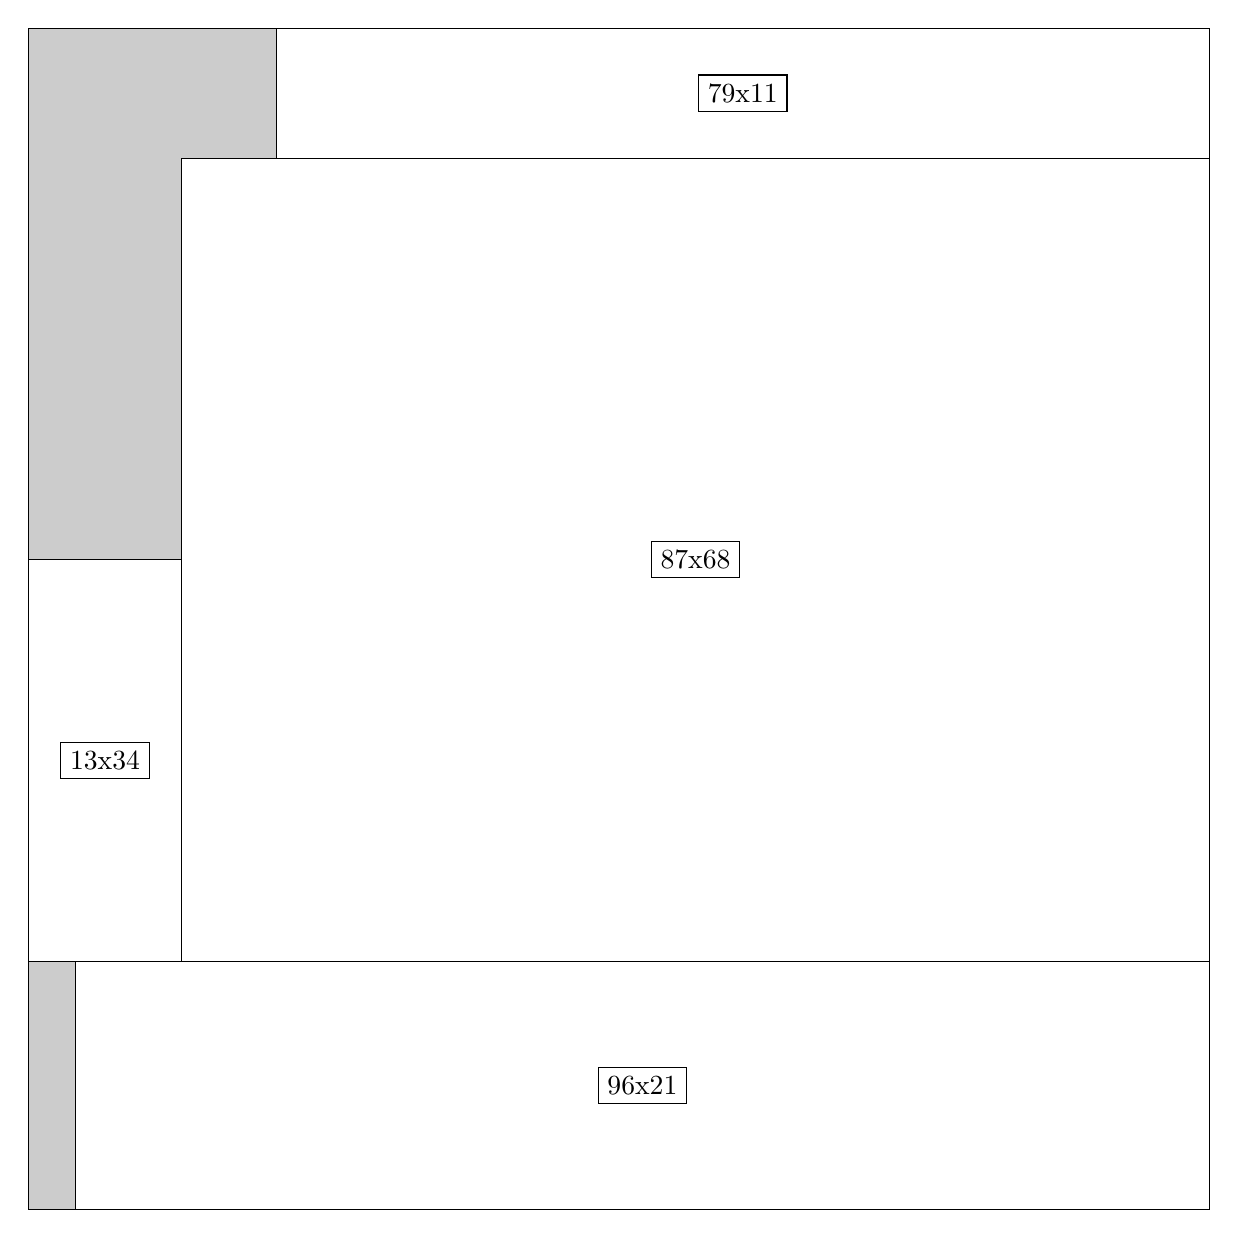
\begin{tikzpicture}[shorten >=1pt,scale=1.0,every node/.style={scale=1.0},->]
\tikzstyle{vertex}=[circle,fill=black!25,minimum size=14pt,inner sep=0pt]
\filldraw[fill=gray!40!white, draw=black] (0,0) rectangle (15.0,15.0);
\foreach \name/\x/\y/\w/\h in {96x21/0.6/0.0/14.399999999999999/3.15,87x68/1.95/3.15/13.049999999999999/10.2,13x34/0.0/3.15/1.95/5.1,79x11/3.15/13.35/11.85/1.65}
\filldraw[fill=white!40!white, draw=black] (\x,\y) rectangle node[draw] (\name) {\name} ++(\w,\h);
\end{tikzpicture}


w =96 , h =21 , x =4 , y =0 , v =2016
\par
w =87 , h =68 , x =13 , y =21 , v =5916
\par
w =13 , h =34 , x =0 , y =21 , v =442
\par
w =79 , h =11 , x =21 , y =89 , v =869
\par
\newpage


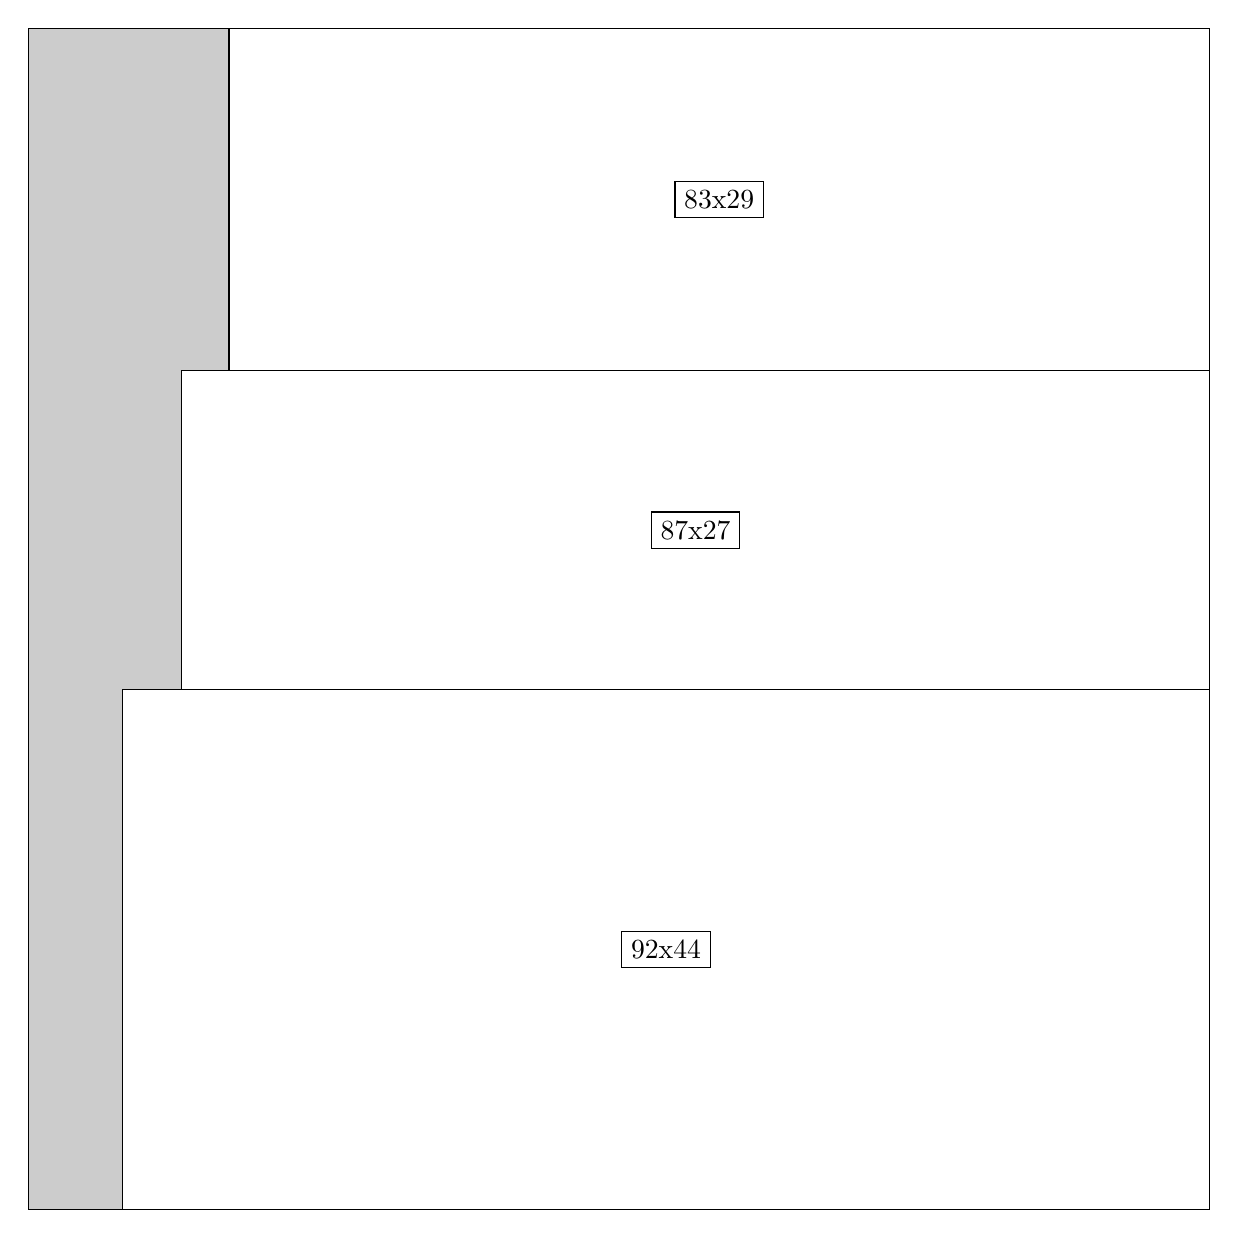
\begin{tikzpicture}[shorten >=1pt,scale=1.0,every node/.style={scale=1.0},->]
\tikzstyle{vertex}=[circle,fill=black!25,minimum size=14pt,inner sep=0pt]
\filldraw[fill=gray!40!white, draw=black] (0,0) rectangle (15.0,15.0);
\foreach \name/\x/\y/\w/\h in {92x44/1.2/0.0/13.799999999999999/6.6,87x27/1.95/6.6/13.049999999999999/4.05,83x29/2.55/10.65/12.45/4.35}
\filldraw[fill=white!40!white, draw=black] (\x,\y) rectangle node[draw] (\name) {\name} ++(\w,\h);
\end{tikzpicture}


w =92 , h =44 , x =8 , y =0 , v =4048
\par
w =87 , h =27 , x =13 , y =44 , v =2349
\par
w =83 , h =29 , x =17 , y =71 , v =2407
\par
\newpage


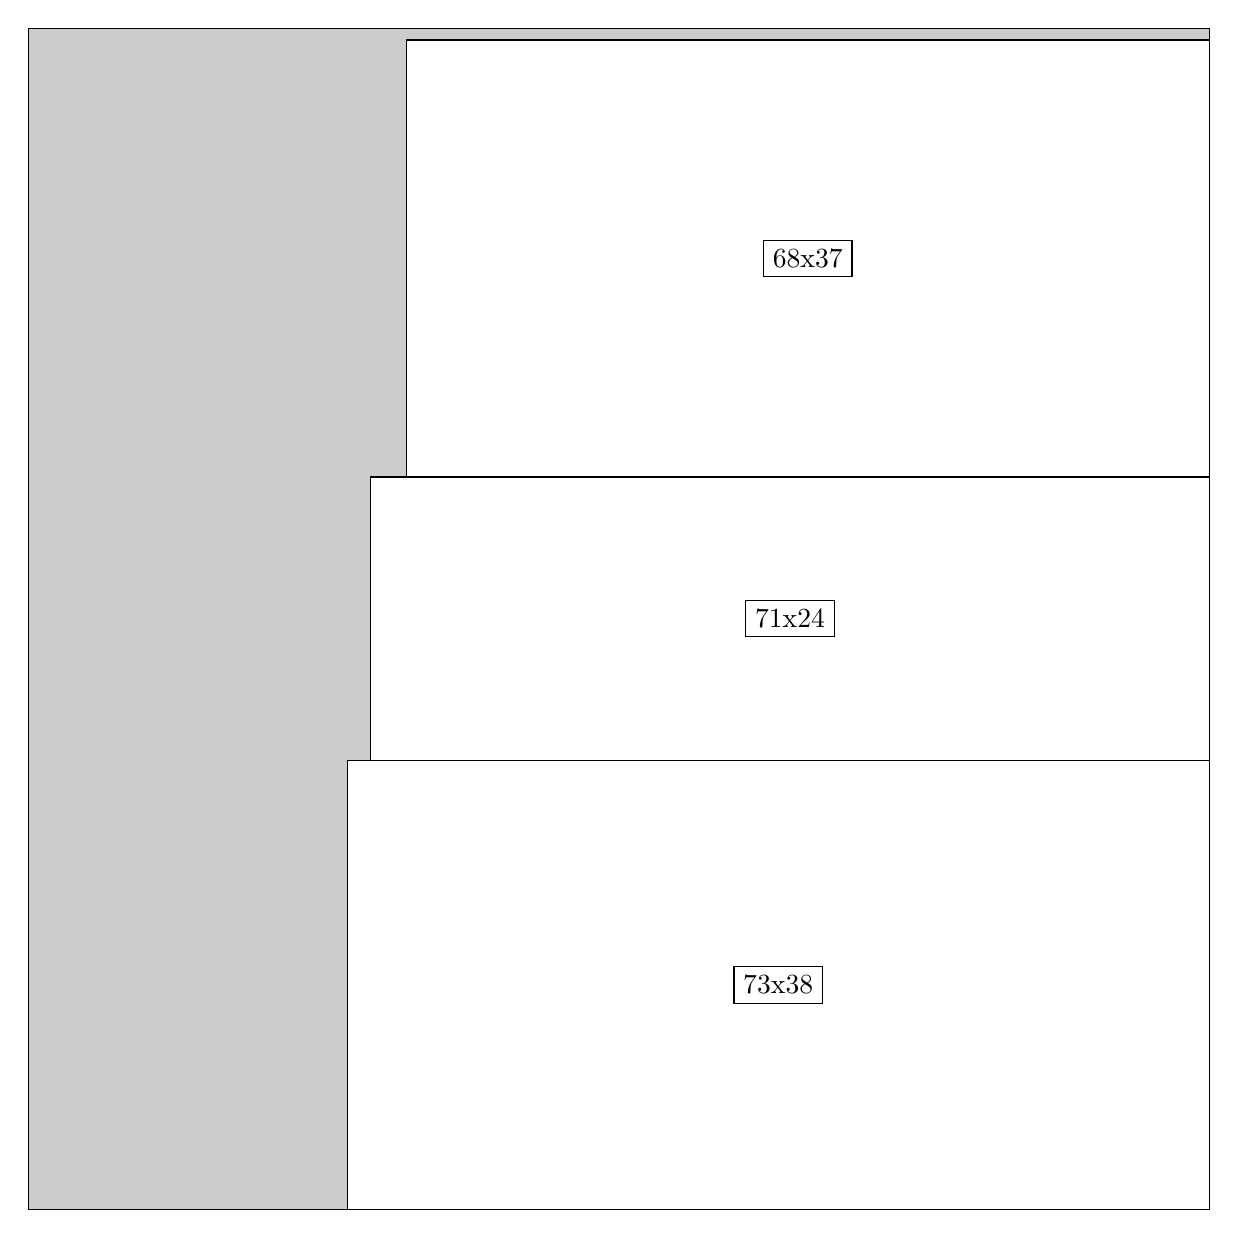
\begin{tikzpicture}[shorten >=1pt,scale=1.0,every node/.style={scale=1.0},->]
\tikzstyle{vertex}=[circle,fill=black!25,minimum size=14pt,inner sep=0pt]
\filldraw[fill=gray!40!white, draw=black] (0,0) rectangle (15.0,15.0);
\foreach \name/\x/\y/\w/\h in {73x38/4.05/0.0/10.95/5.7,71x24/4.35/5.7/10.65/3.5999999999999996,68x37/4.8/9.299999999999999/10.2/5.55}
\filldraw[fill=white!40!white, draw=black] (\x,\y) rectangle node[draw] (\name) {\name} ++(\w,\h);
\end{tikzpicture}


w =73 , h =38 , x =27 , y =0 , v =2774
\par
w =71 , h =24 , x =29 , y =38 , v =1704
\par
w =68 , h =37 , x =32 , y =62 , v =2516
\par
\newpage


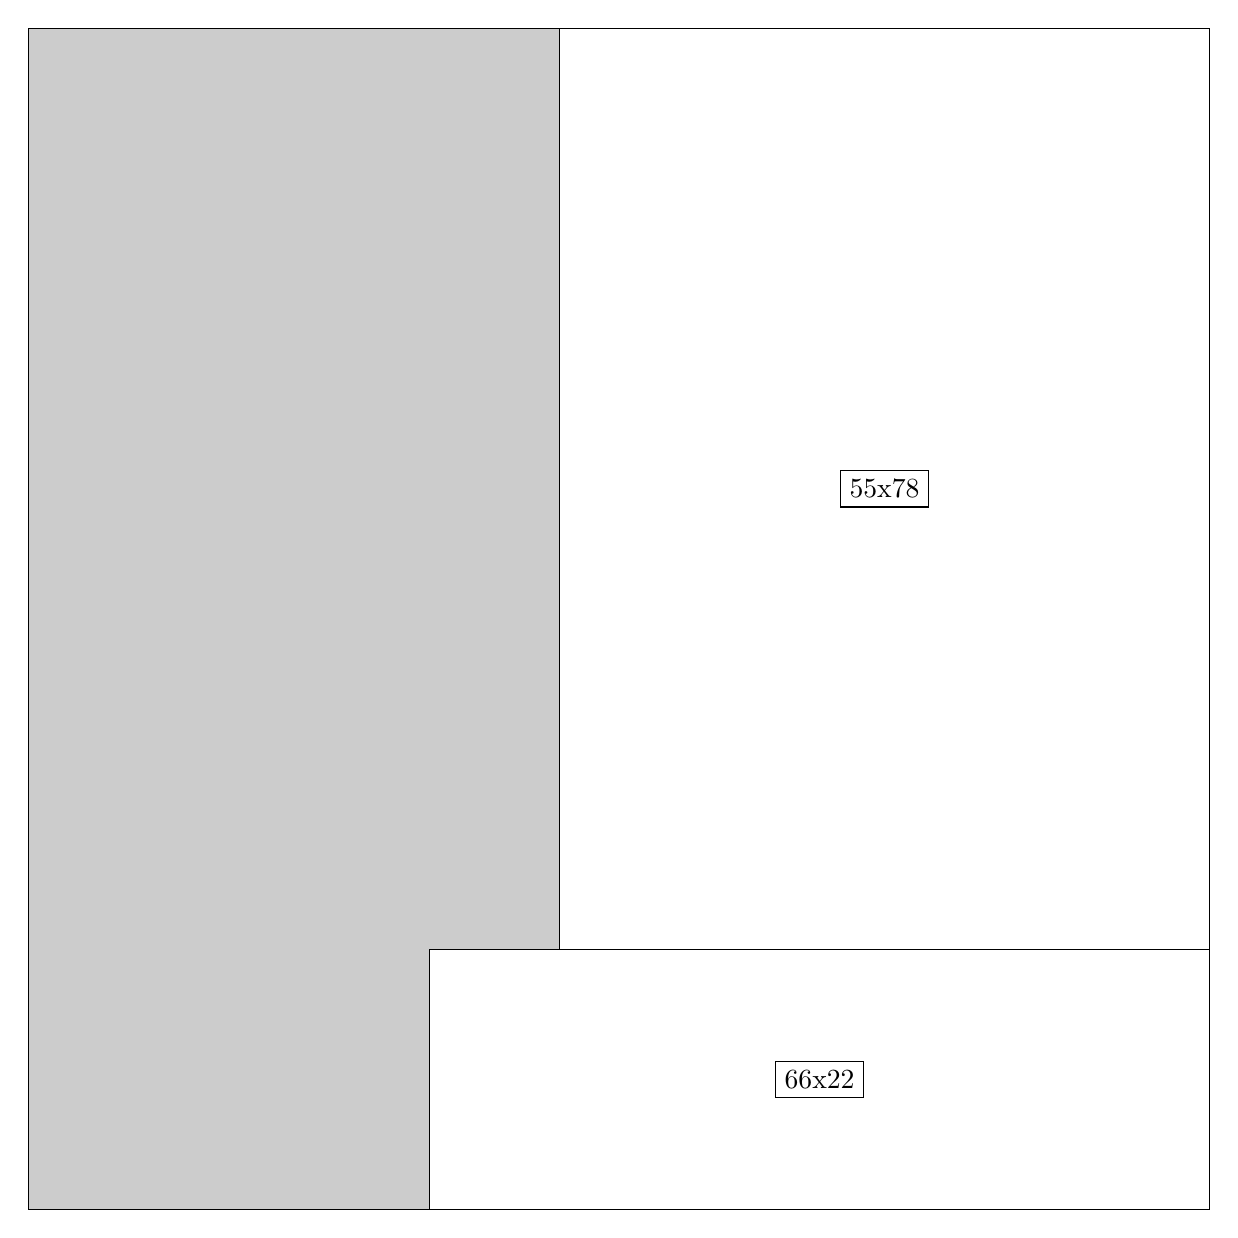
\begin{tikzpicture}[shorten >=1pt,scale=1.0,every node/.style={scale=1.0},->]
\tikzstyle{vertex}=[circle,fill=black!25,minimum size=14pt,inner sep=0pt]
\filldraw[fill=gray!40!white, draw=black] (0,0) rectangle (15.0,15.0);
\foreach \name/\x/\y/\w/\h in {66x22/5.1/0.0/9.9/3.3,55x78/6.75/3.3/8.25/11.7}
\filldraw[fill=white!40!white, draw=black] (\x,\y) rectangle node[draw] (\name) {\name} ++(\w,\h);
\end{tikzpicture}


w =66 , h =22 , x =34 , y =0 , v =1452
\par
w =55 , h =78 , x =45 , y =22 , v =4290
\par
\newpage


\end{document}